% Fonte editável da figura; compilar separadamente com pdflatex.
% O documento principal inclui somente modelo-dados.pdf.
\documentclass[10pt]{article}
\usepackage[T1]{fontenc}
\usepackage[utf8]{inputenc}
\usepackage{lmodern,tikz}
\usepackage[paperwidth=16cm,paperheight=14cm,margin=0cm]{geometry}
\usetikzlibrary{arrows.meta}
\pagestyle{empty}
\setlength{\parindent}{0pt}
\begin{document}
\noindent
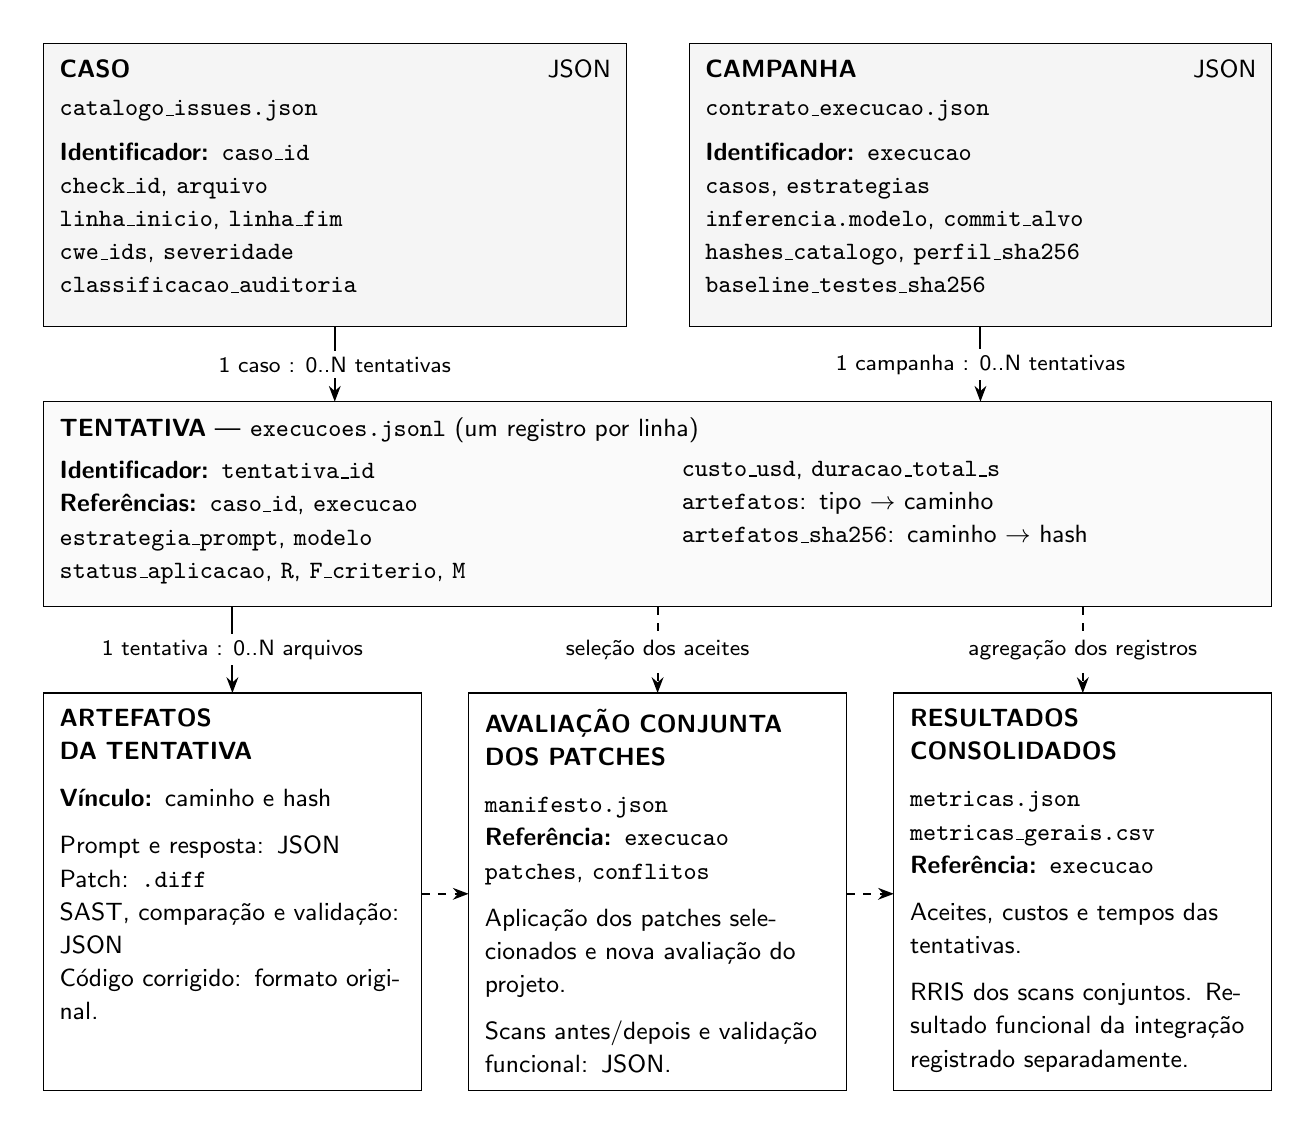
\begin{tikzpicture}[x=1cm,y=1cm,
    every node/.style={font=\sffamily\fontsize{9.5}{12}\selectfont,align=left},
    ref/.style={-{Stealth[length=2mm]},line width=0.7pt},
    deriv/.style={ref,dashed},
    small/.style={font=\sffamily\fontsize{8.5}{10}\selectfont,fill=white,inner sep=2pt}]
\path[use as bounding box] (0,0) rectangle (16,13.8);

% Primeira linha: entidades de referência, com alinhamento simétrico.
\draw[fill=black!4] (0.2,10) rectangle (7.6,13.6);
\node[anchor=north west,text width=7cm,inner sep=0pt] at (0.4,13.4) {
    \textbf{CASO}\hfill JSON\\[2pt]
    \texttt{catalogo\_issues.json}\\[4pt]
    \textbf{Identificador:} \texttt{caso\_id}\\
    \texttt{check\_id}, \texttt{arquivo}\\
    \texttt{linha\_inicio}, \texttt{linha\_fim}\\
    \texttt{cwe\_ids}, \texttt{severidade}\\
    \texttt{classificacao\_auditoria}
};
\draw[fill=black!4] (8.4,10) rectangle (15.8,13.6);
\node[anchor=north west,text width=7cm,inner sep=0pt] at (8.6,13.4) {
    \textbf{CAMPANHA}\hfill JSON\\[2pt]
    \texttt{contrato\_execucao.json}\\[4pt]
    \textbf{Identificador:} \texttt{execucao}\\
    \texttt{casos}, \texttt{estrategias}\\
    \texttt{inferencia.modelo}, \texttt{commit\_alvo}\\
    \texttt{hashes\_catalogo}, \texttt{perfil\_sha256}\\
    \texttt{baseline\_testes\_sha256}
};

% Segunda linha: registro central, com atributos em duas colunas.
\draw[fill=black!2] (0.2,6.45) rectangle (15.8,9.05);
\node[anchor=north west,inner sep=0pt] at (0.4,8.85)
    {\textbf{TENTATIVA} --- \texttt{execucoes.jsonl} (um registro por linha)};
\node[anchor=north west,text width=7.3cm,inner sep=0pt] at (0.4,8.3) {
    \textbf{Identificador:} \texttt{tentativa\_id}\\
    \textbf{Referências:} \texttt{caso\_id}, \texttt{execucao}\\
    \texttt{estrategia\_prompt}, \texttt{modelo}\\
    \texttt{status\_aplicacao}, \texttt{R}, \texttt{F\_criterio}, \texttt{M}
};
\node[anchor=north west,text width=7.3cm,inner sep=0pt] at (8.3,8.3) {
    \texttt{custo\_usd}, \texttt{duracao\_total\_s}\\
    \texttt{artefatos}: tipo $\rightarrow$ caminho\\
    \texttt{artefatos\_sha256}: caminho $\rightarrow$ hash
};

% Terceira linha: arquivos individuais, avaliação conjunta e consolidação.
\draw (0.2,0.3) rectangle (5,5.35);
\node[anchor=north west,text width=4.4cm,inner sep=0pt] at (0.4,5.15) {
    \textbf{ARTEFATOS}\\
    \textbf{DA TENTATIVA}\\[5pt]
    \textbf{Vínculo:} caminho e hash\\[5pt]
    Prompt e resposta: JSON\\
    Patch: \texttt{.diff}\\
    SAST, comparação e validação: JSON\\
    Código corrigido: formato original.
};
\draw (5.6,0.3) rectangle (10.4,5.35);
\node[anchor=north west,text width=4.4cm,inner sep=0pt] at (5.8,5.15) {
    \textbf{AVALIAÇÃO CONJUNTA}\\
    \textbf{DOS PATCHES}\\[5pt]
    \texttt{manifesto.json}\\
    \textbf{Referência:} \texttt{execucao}\\
    \texttt{patches}, \texttt{conflitos}\\[5pt]
    Aplicação dos patches selecionados e nova avaliação do projeto.\\[5pt]
    Scans antes/depois e validação funcional: JSON.
};
\draw (11,0.3) rectangle (15.8,5.35);
\node[anchor=north west,text width=4.4cm,inner sep=0pt] at (11.2,5.15) {
    \textbf{RESULTADOS}\\
    \textbf{CONSOLIDADOS}\\[5pt]
    \texttt{metricas.json}\\
    \texttt{metricas\_gerais.csv}\\
    \textbf{Referência:} \texttt{execucao}\\[5pt]
    Aceites, custos e tempos das tentativas.\\[5pt]
    RRIS dos scans conjuntos. Resultado funcional da integração registrado separadamente.
};

% Referências: cada tentativa pertence a um caso e a uma campanha.
\draw[ref] (3.9,10) -- (3.9,9.05);
\node[small] at (3.9,9.52) {1 caso : 0..N tentativas};
\draw[ref] (12.1,10) -- (12.1,9.05);
\node[small] at (12.1,9.52) {1 campanha : 0..N tentativas};
\draw[ref] (2.6,6.45) -- (2.6,5.35);
\node[small] at (2.6,5.9) {1 tentativa : 0..N arquivos};

% Derivações: não são cardinalidades de entidades persistidas.
\draw[deriv] (8,6.45) -- (8,5.35);
\node[small] at (8,5.9) {seleção dos aceites};
\draw[deriv] (13.4,6.45) -- (13.4,5.35);
\node[small] at (13.4,5.9) {agregação dos registros};
\draw[deriv] (5,2.8) -- (5.6,2.8);
\draw[deriv] (10.4,2.8) -- (11,2.8);
\end{tikzpicture}
\end{document}
